\documentclass[ignorenonframetext,]{beamer}
\setbeamertemplate{caption}[numbered]
\setbeamertemplate{caption label separator}{: }
\setbeamercolor{caption name}{fg=normal text.fg}
\beamertemplatenavigationsymbolsempty
\usepackage{lmodern}
\usepackage{amssymb,amsmath}
\usepackage{ifxetex,ifluatex}
\usepackage{fixltx2e} % provides \textsubscript
\ifnum 0\ifxetex 1\fi\ifluatex 1\fi=0 % if pdftex
  \usepackage[T1]{fontenc}
  \usepackage[utf8]{inputenc}
\else % if luatex or xelatex
  \ifxetex
    \usepackage{mathspec}
  \else
    \usepackage{fontspec}
  \fi
  \defaultfontfeatures{Ligatures=TeX,Scale=MatchLowercase}
\fi
% use upquote if available, for straight quotes in verbatim environments
\IfFileExists{upquote.sty}{\usepackage{upquote}}{}
% use microtype if available
\IfFileExists{microtype.sty}{%
\usepackage{microtype}
\UseMicrotypeSet[protrusion]{basicmath} % disable protrusion for tt fonts
}{}
\newif\ifbibliography
\hypersetup{
            pdftitle={Machine Learning: Chapter 5 - Part I},
            pdfborder={0 0 0},
            breaklinks=true}
\urlstyle{same}  % don't use monospace font for urls
\usepackage{color}
\usepackage{fancyvrb}
\newcommand{\VerbBar}{|}
\newcommand{\VERB}{\Verb[commandchars=\\\{\}]}
\DefineVerbatimEnvironment{Highlighting}{Verbatim}{commandchars=\\\{\}}
% Add ',fontsize=\small' for more characters per line
\usepackage{framed}
\definecolor{shadecolor}{RGB}{248,248,248}
\newenvironment{Shaded}{\begin{snugshade}}{\end{snugshade}}
\newcommand{\KeywordTok}[1]{\textcolor[rgb]{0.13,0.29,0.53}{\textbf{#1}}}
\newcommand{\DataTypeTok}[1]{\textcolor[rgb]{0.13,0.29,0.53}{#1}}
\newcommand{\DecValTok}[1]{\textcolor[rgb]{0.00,0.00,0.81}{#1}}
\newcommand{\BaseNTok}[1]{\textcolor[rgb]{0.00,0.00,0.81}{#1}}
\newcommand{\FloatTok}[1]{\textcolor[rgb]{0.00,0.00,0.81}{#1}}
\newcommand{\ConstantTok}[1]{\textcolor[rgb]{0.00,0.00,0.00}{#1}}
\newcommand{\CharTok}[1]{\textcolor[rgb]{0.31,0.60,0.02}{#1}}
\newcommand{\SpecialCharTok}[1]{\textcolor[rgb]{0.00,0.00,0.00}{#1}}
\newcommand{\StringTok}[1]{\textcolor[rgb]{0.31,0.60,0.02}{#1}}
\newcommand{\VerbatimStringTok}[1]{\textcolor[rgb]{0.31,0.60,0.02}{#1}}
\newcommand{\SpecialStringTok}[1]{\textcolor[rgb]{0.31,0.60,0.02}{#1}}
\newcommand{\ImportTok}[1]{#1}
\newcommand{\CommentTok}[1]{\textcolor[rgb]{0.56,0.35,0.01}{\textit{#1}}}
\newcommand{\DocumentationTok}[1]{\textcolor[rgb]{0.56,0.35,0.01}{\textbf{\textit{#1}}}}
\newcommand{\AnnotationTok}[1]{\textcolor[rgb]{0.56,0.35,0.01}{\textbf{\textit{#1}}}}
\newcommand{\CommentVarTok}[1]{\textcolor[rgb]{0.56,0.35,0.01}{\textbf{\textit{#1}}}}
\newcommand{\OtherTok}[1]{\textcolor[rgb]{0.56,0.35,0.01}{#1}}
\newcommand{\FunctionTok}[1]{\textcolor[rgb]{0.00,0.00,0.00}{#1}}
\newcommand{\VariableTok}[1]{\textcolor[rgb]{0.00,0.00,0.00}{#1}}
\newcommand{\ControlFlowTok}[1]{\textcolor[rgb]{0.13,0.29,0.53}{\textbf{#1}}}
\newcommand{\OperatorTok}[1]{\textcolor[rgb]{0.81,0.36,0.00}{\textbf{#1}}}
\newcommand{\BuiltInTok}[1]{#1}
\newcommand{\ExtensionTok}[1]{#1}
\newcommand{\PreprocessorTok}[1]{\textcolor[rgb]{0.56,0.35,0.01}{\textit{#1}}}
\newcommand{\AttributeTok}[1]{\textcolor[rgb]{0.77,0.63,0.00}{#1}}
\newcommand{\RegionMarkerTok}[1]{#1}
\newcommand{\InformationTok}[1]{\textcolor[rgb]{0.56,0.35,0.01}{\textbf{\textit{#1}}}}
\newcommand{\WarningTok}[1]{\textcolor[rgb]{0.56,0.35,0.01}{\textbf{\textit{#1}}}}
\newcommand{\AlertTok}[1]{\textcolor[rgb]{0.94,0.16,0.16}{#1}}
\newcommand{\ErrorTok}[1]{\textcolor[rgb]{0.64,0.00,0.00}{\textbf{#1}}}
\newcommand{\NormalTok}[1]{#1}
\usepackage{longtable,booktabs}
\usepackage{caption}
% These lines are needed to make table captions work with longtable:
\makeatletter
\def\fnum@table{\tablename~\thetable}
\makeatother
\usepackage{graphicx,grffile}
\makeatletter
\def\maxwidth{\ifdim\Gin@nat@width>\linewidth\linewidth\else\Gin@nat@width\fi}
\def\maxheight{\ifdim\Gin@nat@height>\textheight0.8\textheight\else\Gin@nat@height\fi}
\makeatother
% Scale images if necessary, so that they will not overflow the page
% margins by default, and it is still possible to overwrite the defaults
% using explicit options in \includegraphics[width, height, ...]{}
\setkeys{Gin}{width=\maxwidth,height=\maxheight,keepaspectratio}

% Prevent slide breaks in the middle of a paragraph:
\widowpenalties 1 10000
\raggedbottom

\AtBeginPart{
  \let\insertpartnumber\relax
  \let\partname\relax
  \frame{\partpage}
}
\AtBeginSection{
  \ifbibliography
  \else
    \let\insertsectionnumber\relax
    \let\sectionname\relax
    \frame{\sectionpage}
  \fi
}
\AtBeginSubsection{
  \let\insertsubsectionnumber\relax
  \let\subsectionname\relax
  \frame{\subsectionpage}
}

\setlength{\parindent}{0pt}
\setlength{\parskip}{6pt plus 2pt minus 1pt}
\setlength{\emergencystretch}{3em}  % prevent overfull lines
\providecommand{\tightlist}{%
  \setlength{\itemsep}{0pt}\setlength{\parskip}{0pt}}
\setcounter{secnumdepth}{0}
\setbeamertemplate{navigation symbols}{}
\setbeamertemplate{footline}[page number]

\title{Machine Learning: Chapter 5 - Part I}
\subtitle{Missing Values Revisited}
\date{}

\begin{document}
\frame{\titlepage}

\begin{frame}{Notations}

Supervised Learning Model

\[Y = f(\bold{X}) + \varepsilon\]

Where

\begin{itemize}
\tightlist
\item
  \(Y:=\) target feature
\item
  \(\bold{X}:=\) descriptive features
\item
  \(\varepsilon:=\) error term
\item
  \(f(\bold{X}):=\) unknown functional form
\end{itemize}

\end{frame}

\begin{frame}{Possible combinations}

Given an observation \(i\),

\begin{enumerate}
\def\labelenumi{\arabic{enumi}.}
\tightlist
\item
  \(Y_{i}\) is missing but \(\bold{X}_{i}\) is intact or some of
  \(\bold{X}_{i}\) are missing
\item
  \(Y_{i}\) is not missing but some of \(\bold{X}_{i}\) are missing
\item
  \(Y_{i}\) is not missing but \textbf{all} \(\bold{X}_{i}\) are missing
\item
  Both \(Y_{i}\) and \(\bold{X}_{i}\) are not missing
\end{enumerate}

\begin{itemize}
\tightlist
\item
  Delete row \(i\) for Case 3, as it is probably an error
\item
  Case 4 is ideal \emph{if} we have 90 to 95 \% of such type in the data
\item
  Let's discuss and \emph{attempt} to solve Case 1 and Case 2
\end{itemize}

\end{frame}

\begin{frame}{Case 1: Missing values in target feature \(Y_{i}\)}

\begin{itemize}
\tightlist
\item
  You cannot train the model when \(Y_{i}\) is missing
\item
  Ask why \(Y_{i}\) is missing
\item
  \(\implies\) Could it be due to transformation?
\item
  Example: \(\log{y}\) when \(y=0\)
\item
  Keep it as part of test model but no evaluation
\item
  Predict it! Isn't it a data science job?
\end{itemize}

\end{frame}

\begin{frame}[fragile]{Case 1: \(Y_{i}\) is categorical}

\begin{itemize}
\tightlist
\item
  Example: iris
\end{itemize}

\begin{Shaded}
\begin{Highlighting}[]
\OperatorTok{>}\StringTok{ }\KeywordTok{data}\NormalTok{(iris)}
\OperatorTok{>}\StringTok{ }\KeywordTok{levels}\NormalTok{(iris}\OperatorTok{$}\NormalTok{Species)}
\end{Highlighting}
\end{Shaded}

\begin{verbatim}
## [1] "setosa"     "versicolor" "virginica"
\end{verbatim}

\begin{itemize}
\tightlist
\item
  What if \texttt{setosa} is taken out?
\item
  Without prior knowledge, are there three or four or five species?
\item
  Even with prior knowledge, you cannot train models without target
  values where \texttt{species\ =\ setosa}.
\item
  Possible solution: Cluster analysis (Unsupervised Learning)
\item
  Idea: hope that unsupervised learners would produce three respectives
  clusters for three species
\item
  Suggested course:
  \href{http://www1.rmit.edu.au/courses/051637}{COSC2670 Practical Data
  Science}
\end{itemize}

\end{frame}

\begin{frame}{Case 1: \(Y_{i}\) is discrete}

\begin{itemize}
\tightlist
\item
  Example: \(Y:=\) count of wombats in Building 10
\item
  \(Y_{i}=0, 1, 2, 3, 4, 5, ...\)
\item
  Does \(Y_{i}=0\) mean missing value or actual zero count?
\item
  If there are excess zeroes, consider Zero-Inflated Poisson (ZIP) Model
\item
  Two zero generating processes:
\end{itemize}

\begin{enumerate}
\def\labelenumi{\arabic{enumi}.}
\tightlist
\item
  A binary distribution that generates structural zeros.
\item
  A Poisson distribution that generates counts which may be zero
\end{enumerate}

\begin{itemize}
\tightlist
\item
  Suggested course:
  \href{http://www1.rmit.edu.au/courses/011998}{MATH1298: Analysis of
  Categorical Data}
\end{itemize}

\end{frame}

\begin{frame}{Case 2: Missing values in \(\bold{X}_{i}\)}

Types of missing values

\begin{enumerate}
\def\labelenumi{\arabic{enumi}.}
\tightlist
\item
  Missing Completely At Random (MCAR)
\item
  Missing At Random (MAR)
\item
  \color{red}Missing Not At Random (MNAR) \color{black}
\end{enumerate}

\begin{itemize}
\tightlist
\item
  Types 1 and 2 are okay
\item
  Type 3 is problematic (no solution)
\end{itemize}

\end{frame}

\begin{frame}{Case 2: Example}

\begin{itemize}
\tightlist
\item
  \(X_{1}:=\) Heart Rate
\item
  \(X_{2}:=\) Calories Burnt
\item
  Number of observations = 30
\item
  MCAR: randomly remove \(X_{2}\)
\item
  MAR: keep \(X_{2}\) when \(X_{1} > 65\)
\item
  MNAR: remove \(X_{2}\) when \(X_{2} > 120\)
\end{itemize}

\end{frame}

\begin{frame}{Case 2: First 10 observations of the example}

\begin{longtable}[]{@{}rrrrr@{}}
\toprule
heartRate & CaloriesBurnt & MCAR & MAR & MNAR\tabularnewline
\midrule
\endhead
69.39524 & 116.4480 & NA & 116.4480 & NA\tabularnewline
72.69823 & 121.2844 & 121.2844 & 121.2844 & 121.2844\tabularnewline
90.58708 & 118.7665 & 118.7665 & 118.7665 & NA\tabularnewline
75.70508 & 118.2623 & 118.2623 & 118.2623 & NA\tabularnewline
76.29288 & 115.2419 & 115.2419 & 115.2419 & NA\tabularnewline
92.15065 & 119.7749 & 119.7749 & 119.7749 & NA\tabularnewline
79.60916 & 116.0755 & 116.0755 & 116.0755 & NA\tabularnewline
62.34939 & 111.6603 & 111.6603 & NA & NA\tabularnewline
68.13147 & 118.0989 & 118.0989 & 118.0989 & NA\tabularnewline
70.54338 & 124.5950 & 124.5950 & 124.5950 & 124.5950\tabularnewline
\bottomrule
\end{longtable}

\end{frame}

\begin{frame}{Case 2: MCAR}

\begin{itemize}
\tightlist
\item
  Missingness does not depend on data
\item
  \(\implies\) Missingness of \(X_{2}\) is not related to \(X_{1}\)
  (other variable)
\item
  \(\implies\) Missingness of \(X_{2}\) is not related to \(X_{2}\)
  (itself)
\item
  \(P(\text{Missingness}|X_{2}) = P(\text{Missingness})\)
\item
  How to detect it? Conduct t-test to assess mean difference in
  \(X_{1}\):
\end{itemize}

\[X_{1} | X_{2} \text{ is not missing vs } X_{1} | X_{2} \text{ is  missing}\]

\begin{itemize}
\tightlist
\item
  Conclusion: it is likely MCAR if \(H_0\) cannot be rejected.
\item
  Problem: what if there are more than 2 variables?
\end{itemize}

\end{frame}

\begin{frame}{Case 2: MAR and MNAR}

\textbf{MAR}

\begin{itemize}
\tightlist
\item
  Missingness depends only on observed data
\item
  \(\implies\) Missingness of \(X_{2}\) is \textbf{related} to \(X_{1}\)
  (other variable)
\end{itemize}

\textbf{MNAR}

\begin{itemize}
\tightlist
\item
  Missingness depends only on missing data
\item
  \(\implies\) Missingness of \(X_{2}\) is \textbf{related} to \(X_{2}\)
  (itself)
\end{itemize}

\textbf{Issues}

\begin{itemize}
\tightlist
\item
  In practice, it is difficult to distinguish MAR adn MNAR
\item
  If you have prior knowledge about MNAR (i.e.~you know why it is
  missing), mitigate it by asking for pre-processed data from data owner
\item
  If you have no prior knowledge or you cannot mitigate MNAR, assume it
  is MAR
\end{itemize}

\end{frame}

\begin{frame}{Case 2: Solution?}

\begin{itemize}
\tightlist
\item
  No complete solution; you can only mitigate it
\item
  Recall: data processing cannot add new information
\item
  MCAR: ``Complete-Case'' Analysis
\item
  MAR: Imputation Methods
\item
  MNAR: No solution. Risky solution is to assume it is MAR
\item
  Practice, you can use methods who mitigate MAR on MCAR, but the
  reverse is not true
\end{itemize}

\end{frame}

\begin{frame}[fragile]{Case 2: Complete-Case Analysis}

\begin{itemize}
\tightlist
\item
  Delete the rows if the number of complete cases \(>=95\%\)
\item
  In R use \texttt{complete.cases} to check number of complete cases
\item
  In R use \texttt{na.omit} to remove missing rows
\item
  Side effect: \color{red}{waste of information}
\item
  Unknown side effect: \color{red}{introduces bias if MAR}
\end{itemize}

\end{frame}

\begin{frame}[fragile]{Case 2: Complete-Case Analysis Example}

\begin{itemize}
\tightlist
\item
  Consider \texttt{heartRate} and \texttt{MCAR}
\end{itemize}

\begin{Shaded}
\begin{Highlighting}[]
\OperatorTok{>}\StringTok{ }\NormalTok{data <-}\StringTok{ }\KeywordTok{read.csv}\NormalTok{(}\StringTok{'heartRateAndCaloriesBurnt.csv'}\NormalTok{)}
\OperatorTok{>}\StringTok{ }\NormalTok{df   <-}\StringTok{ }\NormalTok{data[, }\KeywordTok{c}\NormalTok{(}\StringTok{'heartRate'}\NormalTok{, }\StringTok{'MCAR'}\NormalTok{)]}
\OperatorTok{>}\StringTok{ }\KeywordTok{sum}\NormalTok{(  }\KeywordTok{complete.cases}\NormalTok{( df ) )}
\end{Highlighting}
\end{Shaded}

\begin{verbatim}
## [1] 93
\end{verbatim}

\begin{itemize}
\tightlist
\item
  93 complete cases out of 100 observations. This is not so bad
\item
  Remove \texttt{NA} rows and calculate the number of rows
\end{itemize}

\begin{Shaded}
\begin{Highlighting}[]
\OperatorTok{>}\StringTok{ }\NormalTok{df  <-}\StringTok{ }\KeywordTok{na.omit}\NormalTok{(df)}
\OperatorTok{>}\StringTok{ }\KeywordTok{nrow}\NormalTok{(df)}
\end{Highlighting}
\end{Shaded}

\begin{itemize}
\tightlist
\item
  Try with \texttt{MNAR} and \texttt{MAR}.
\end{itemize}

\end{frame}

\begin{frame}{Case 2: Single imputation overview}

\begin{longtable}[]{@{}lrr@{}}
\toprule
Imputation & Difficulty & Accuracy\tabularnewline
\midrule
\endhead
Unconditional Mean/Median/Mode & 1 & 1\tabularnewline
Unconditional Distribution & 2 & 2\tabularnewline
Conditional Mean & 3 & 3\tabularnewline
Conditional Distribution & 4 & 4\tabularnewline
\bottomrule
\end{longtable}

\end{frame}

\begin{frame}[fragile]{Case 2: Single imputation method and issues (Part
I)}

\textbf{Unconditional Mean/Median/Mode}

\begin{itemize}
\tightlist
\item
  In R, use \texttt{mean(x,\ na.rm\ =\ FALSE)}
\item
  \color{red}{Issue: Zero variance in imputed values}
\end{itemize}

\textbf{Unconditional Distribution}

\begin{itemize}
\tightlist
\item
  Hot deck encoding: impute with a randomly choosen one non-missing
  value
\item
  \color{red}{Issue: less biased variance in imputed values, wrong correlation}
\end{itemize}

\end{frame}

\begin{frame}[fragile]{Case 2: Single imputation method and issues (Part
II)}

\textbf{Conditional Mean}

\begin{itemize}
\item
  Use linear regression to impute missing values
\item
  Example in \texttt{R}
\item
  Other regression methods also work
\item
  R package: \texttt{missForest} (not recommended as we have
  \texttt{mlr})
\item
  \color{red}{Issue: wrong conditional variance}
\end{itemize}

\textbf{Conditional Distribution}

\begin{itemize}
\tightlist
\item
  Add some random noises to linear regression
\item
  \color{red}{How to generate random noises}
\end{itemize}

\end{frame}

\begin{frame}{Case 2: Single imputation visualisation}

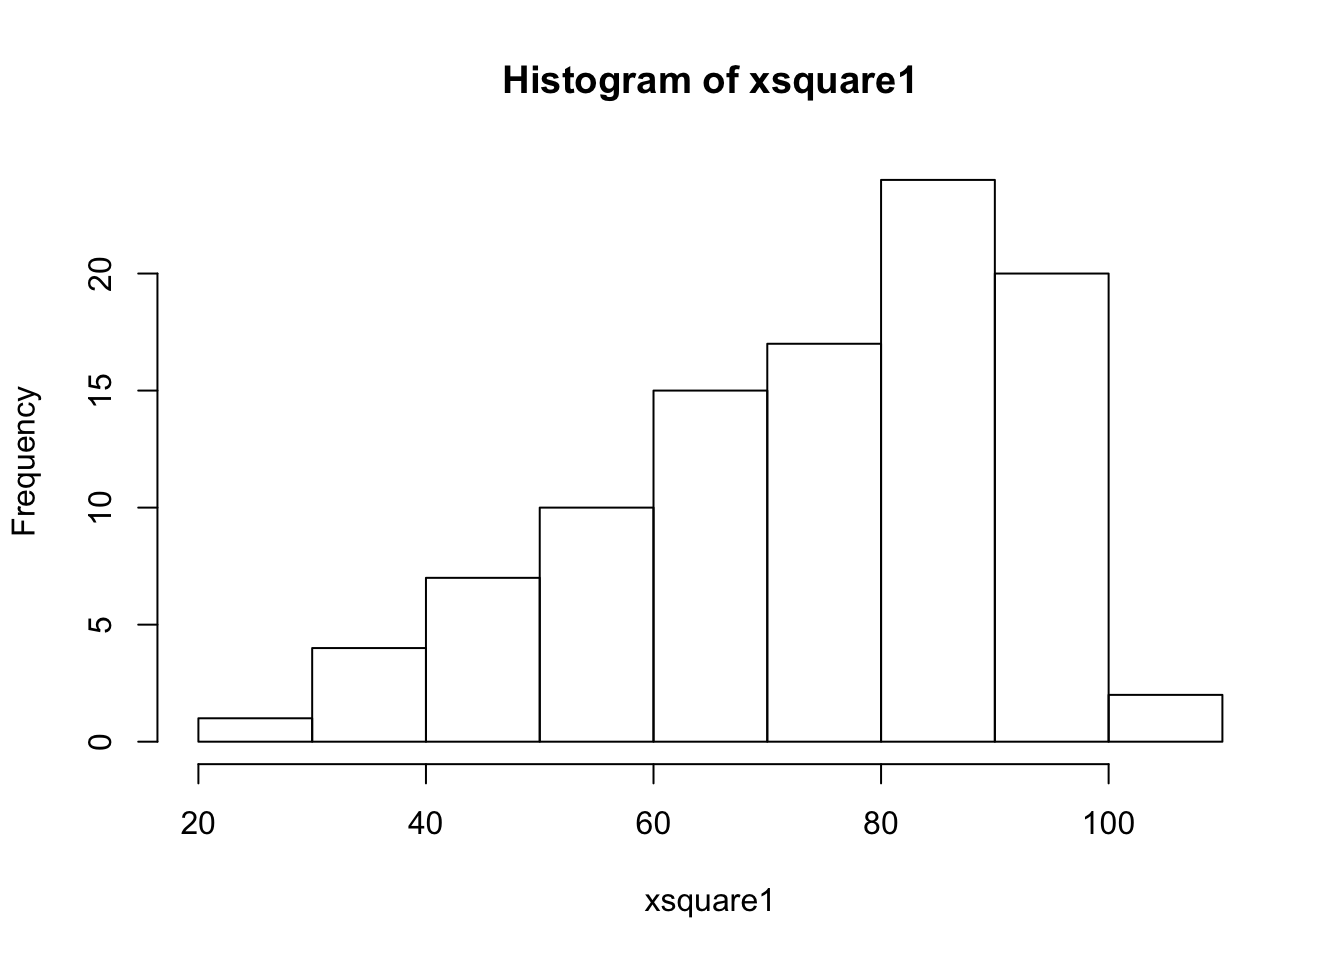
\includegraphics{4_Weekly_Presentation_PDF_files/figure-beamer/unnamed-chunk-7-1.pdf}

\end{frame}

\begin{frame}[fragile]{Case 2: Imputation with \texttt{mlr}: An Example}

\begin{itemize}
\tightlist
\item
  Data: \texttt{weightTypes}
\item
  \(n:=100\)
\item
  Descriptive Features:
\end{itemize}

\begin{enumerate}
\def\labelenumi{\arabic{enumi}.}
\tightlist
\item
  \texttt{heartRate}
\item
  \texttt{CaloriesBurnt}
\item
  \texttt{numberOfMealsPerDay}
\item
  \texttt{gender}
\item
  \texttt{exerciseIntensity}
\end{enumerate}

\begin{itemize}
\tightlist
\item
  Target feature = \texttt{weightType}
\end{itemize}

\end{frame}

\begin{frame}[fragile]{Case 2: Unconditional mean imputation with
\texttt{mlr}}

\begin{itemize}
\tightlist
\item
  Impute by variable types
\end{itemize}

\begin{Shaded}
\begin{Highlighting}[]
\KeywordTok{library}\NormalTok{(mlr)}
\NormalTok{data2   <-}\StringTok{ }\KeywordTok{read.csv}\NormalTok{(}\StringTok{'weightTypes.csv'}\NormalTok{)}
\NormalTok{impute1 <-}\StringTok{ }\KeywordTok{impute}\NormalTok{(data2, }\DataTypeTok{target =} \StringTok{'weightType'}\NormalTok{, }
                  \DataTypeTok{classes =} \KeywordTok{list}\NormalTok{(}\DataTypeTok{numeric =} \KeywordTok{imputeMean}\NormalTok{(),}
                                 \DataTypeTok{factor  =} \KeywordTok{imputeMode}\NormalTok{(),}
                                 \DataTypeTok{integer =} \KeywordTok{imputeMedian}\NormalTok{())}
\NormalTok{                  )}
\end{Highlighting}
\end{Shaded}

\begin{itemize}
\tightlist
\item
  Get the imputed data set via \texttt{impute1\$data}
\item
  Get information via \texttt{impute1\$desc}
\end{itemize}

\end{frame}

\begin{frame}[fragile]{Case 2: Conditional mean with \texttt{mlr}}

\begin{itemize}
\tightlist
\item
  Impute selected columns
\item
  Let's try decision tree on \texttt{exerciseIntensity}
\end{itemize}

\begin{Shaded}
\begin{Highlighting}[]
\KeywordTok{impute}\NormalTok{(data2, }\DataTypeTok{target =} \StringTok{'weightType'}\NormalTok{, }
       \DataTypeTok{cols =} \KeywordTok{list}\NormalTok{(}
         \DataTypeTok{CaloriesBurnt       =} \KeywordTok{imputeNormal}\NormalTok{(),}
         \DataTypeTok{numberOfMealsPerDay =} \KeywordTok{imputeMedian}\NormalTok{(),}
         \DataTypeTok{gender              =} \KeywordTok{imputeMode}\NormalTok{(),}
         \DataTypeTok{exerciseIntensity   =} \KeywordTok{imputeLearner}\NormalTok{(}\StringTok{"classif.rpart"}\NormalTok{))}
\NormalTok{)}
\end{Highlighting}
\end{Shaded}

\end{frame}

\begin{frame}[fragile]{Case 2: Which learners offer imputations?}

For regression,

\begin{itemize}
\tightlist
\item
  \texttt{listLearners("regr",\ properties\ =\ "missings"){[}c("class",\ "package"){]}}
\end{itemize}

For classification,

\begin{itemize}
\tightlist
\item
  \texttt{listLearners("classif",\ properties\ =\ "missings"){[}c("class",\ "package"){]}}
\end{itemize}

\end{frame}

\begin{frame}[fragile]{Case 2: Sneak peek to multiple imputation}

\textbf{Problems of Single Imputation}

\begin{itemize}
\tightlist
\item
  Too optimistic: Imputation model is an estimation, but not the true
  model
\item
  \(\implies\) imputed values have some uncertainty
\item
  Solution: Multiple Imputation
\end{itemize}

\textbf{Multiple Imputation}

\begin{itemize}
\tightlist
\item
  Beyond scope of MATH2319
\item
  Not recommended in the project
\item
  R Package: \texttt{mice} (Multivariate Imputation by Chained
  Equations)
\item
  It is based on Gibbs Sampler
\item
  Recommended course:
  \href{http://www1.rmit.edu.au/courses/050645}{MATH2269 Applied
  Bayesian Statistics}
\end{itemize}

\end{frame}

\begin{frame}[fragile]{Summary}

\begin{itemize}
\tightlist
\item
  Missing values in target features vs descriptive features
\item
  Be pragmatic, use the right tools
\item
  Types of missing values in descriptive features
\item
  Key R functions to know: \texttt{mlr:impute} and
  \texttt{complete.cases}
\end{itemize}

\end{frame}

\end{document}
